\documentclass[11pt]{article}
\usepackage{setspace}
\usepackage{hyperref}
\usepackage[utf8]{inputenc}
\usepackage[T1]{fontenc}
\usepackage{fullpage}
\usepackage{amsmath}
\usepackage{amssymb,amsfonts}
\usepackage[all,arc]{xy}
\usepackage{enumitem}
\usepackage{mathrsfs}
\usepackage{bbm}
\usepackage{graphicx}
\usepackage{subfiles}
\usepackage{setspace}
\usepackage{float}
\usepackage{subcaption}
\usepackage{verbatim}
\usepackage{listings}
\setlength{\footskip}{40pt}
\graphicspath{{Figures/}}
\numberwithin{figure}{section}
\setlength\parindent{0pt}

\begin{document}
%\doublespacing
\begin{titlepage}
\begin{center} 
\vspace*{2cm}
\textsc{\huge Project Requirements}\\[1cm]
\textsc{\LARGE Phase Factor}\\[13cm]

\textsc{\large Matthew Arendall}\\[0.2cm]
\textsc{\large Bryan DiLaura} \\[0.2cm]
\textsc{\large Ariel Hoffman} \\[0.2cm]
\textsc{\large Andrew Kee} \\[0.2cm]
\textsc{\large Ryan Montoya} \\[0.2cm]
\textsc{\large Jonathan Quinn} \\[0.2cm]

\end{center}
\end{titlepage}
\vfill

\pagebreak

\tableofcontents
\pagebreak

\section{Responsibilities, Roles, and Components}
\subfile{PhasedArray}
\pagebreak
\subfile{AndroidApplication}
\pagebreak
\subfile{SoftwareDefinedRadio}

\section{System Diagrams}
\subsection{Transmit}
	\begin{figure}[H]
		\centering
		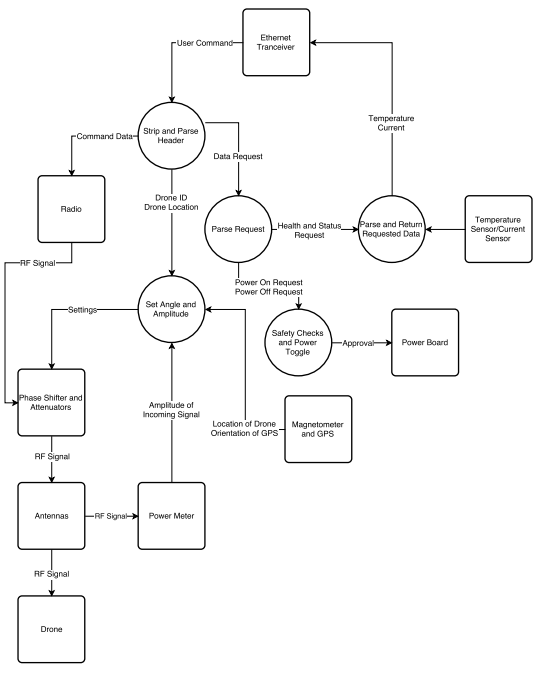
\includegraphics[scale=1]{../SystemDiagram/Transmit.png}
		\caption{System Diagram in Transmit Mode \label{fig:System Diagram in Transmit Mode}}
	\end{figure}
\subsection{Receive}
	\begin{figure}[H]
		\centering
		\includegraphics[scale=1]{../SystemDiagram/Receive.png}
		\caption{Transmit Diagram in Receive Mode \label{fig:Transmit Diagram in Receive Mode}}
	\end{figure}
\end{document}








